\startappendix{Additional Information}
\label{chapter:appendix}
Detailed data value for Figure \ref{fig:5.4}
\begin{eqnarray} 
\resizebox{0.9\linewidth}{!}{$
\begin{bmatrix}
0& 0& 0& 0& 0& 0& 0& 0& 0& 0& 0& 0.299586& 0& 0& 0& 0& 0& 0\\
0& 0& 0& 0.664053& 0& 0& 0& 0& 0& 0& 0& 0& 0& 0& 0& 0& 0& 0\\
0& 0& 0& 0& 0& 0& 0& 0& 0& 0& 0& 0& 0& 0& 0& 0& 0.021196& 0\\
0& 0& 0& 0& 0& 0& 0& 0& 0.00662804& 0& 0& 0& 0& 0& 0& 0& 0& 0\\
0& 0& 0& 0& 0& 0& 0& 0& 0& 0& 0& 0& 0.000642609& 0& 0& 0& 0& 0\\
0& 0& 0& 0& 0& 0& 0& 0& 0& 0& 0& 0& 0.00789& 0& 0& 0& 0& 0
\end{bmatrix}
$}
\label{eqn:A.1}
\end{eqnarray}

Detailed data value for Figure \ref{fig:5.5}
\begin{eqnarray}
\resizebox{0.9\linewidth}{!}{$
\begin{bmatrix}
0& 0& 0& 0& 0& 0& 0.299586& 0& 0& 0& 0& 0& 0& 0& 0& 0& 0& 0\\
0& 0& 0& 0.664053& 0& 0& 0& 0& 0& 0& 0& 0& 0& 0& 0& 0& 0& 0\\
0& 0.021196& 0& 0& 0& 0& 0& 0& 0& 0& 0& 0& 0& 0& 0& 0& 0& 0\\
0& 0& 0& 0& 0& 0& 0& 0& 0.00662804& 0& 0& 0& 0& 0& 0& 0& 0& 0\\
0& 0& 0& 0& 0& 0.000642609& 0& 0& 0& 0& 0& 0& 0& 0& 0& 0& 0& 0\\
0& 0& 0& 0& 0& 0.00789& 0& 0& 0& 0& 0& 0& 0& 0& 0& 0& 0& 0
\end{bmatrix}
$}
\label{eqn:A.2}
\end{eqnarray}

Detailed data value for Figure \ref{fig:5.6}
\begin{eqnarray}
\resizebox{0.9\linewidth}{!}{$
\begin{bmatrix}
0& 0& 0& 0& 0& 0& 0& 0& 0& 0& 0& 0.299586& 0& 0& 0& 0& 0& 0\\
0& 0& 0& 0.664053& 0& 0& 0& 0& 0& 0& 0& 0& 0& 0& 0& 0& 0& 0\\
0& 0& 0& 0& 0& 0& 0& 0& 0& 0& 0& 0& 0& 0& 0& 0& 0.021196& 0\\
0& 0& 0& 0& 0& 0& 0& 0& 0.00662804& 0& 0& 0& 0& 0& 0& 0& 0& 0\\
0& 0& 0& 0& 0& 0& 0& 0& 0& 0& 0& 0& 0.000642609& 0& 0& 0& 0& 0\\
0& 0& 0& 0& 0& 0& 0& 0& 0& 0& 0& 0& 0.00789& 0& 0& 0& 0& 0
\end{bmatrix}
$}
\label{eqn:A.3}
\end{eqnarray}


Detailed data value for Figure \ref{fig:6.1}
\begin{eqnarray}
\resizebox{0.5\linewidth}{!}{$
\begin {bmatrix}
0& 0& 0& 0& 0& 0& 0& 0.03218& 0 \\
0& 0.73929& 0& 0& 0& 0& 0& 0& 0 \\
0& 0& 0& 0.19745& 0& 0& 0& 0& 0 \\
0.00173& 0& 0& 0& 0& 0& 0& 0& 0 \\
0& 0& 0& 0& 0& 0& 0& 0.01819& 0 \\ 
0& 0& 0& 0& 0& 0& 0.01116& 0& 0
\end {bmatrix} 
$}
\label{eqn:A.4}
\end{eqnarray}

Detailed data value for Figure \ref{fig:6.2}
\begin{eqnarray}
\resizebox{0.5\linewidth}{!}{$
\begin {bmatrix}
0& 0& 0& 0& 0& 0& 0& 0.019308& 0 \\
0& 0.443574& 0& 0& 0& 0& 0& 0& 0 \\
0& 0& 0& 0.11847& 0& 0& 0& 0& 0  \\
0.001038& 0& 0& 0& 0& 0& 0& 0& 0 \\ 
0& 0& 0& 0& 0& 0& 0& 0.010914& 0 \\
0& 0& 0& 0& 0& 0& 0.006696& 0& 0 \\
0.4
\end {bmatrix}
$}
\label{eqn:A.5}
\end{eqnarray}

Detailed data value for Figure \ref{fig:6.4}. Target composition
\begin{eqnarray}
\resizebox{0.9\linewidth}{!}{$
\begin {bmatrix}
& 0& 0& 0& 0& 0.53762& 0& 0& 0& 0& 0& 0& 0& 0& 0& 0& 0& 0 \\
0& 0& 0.26894& 0& 0& 0& 0& 0& 0& 0& 0& 0& 0& 0& 0& 0& 0& 0 \\
0& 0& 0& 0& 0& 0& 0& 0& 0& 0& 0.03951& 0& 0& 0& 0& 0& 0& 0 \\
0& 0& 0& 0& 0& 0& 0& 0& 0& 0& 0& 0& 0& 0& 0& 0.11382& 0& 0 \\ 
0& 0& 0& 0& 0.01604& 0& 0& 0& 0& 0& 0& 0& 0& 0& 0& 0& 0& 0 \\
0& 0& 0.02407& 0& 0& 0& 0& 0& 0& 0& 0& 0& 0& 0& 0& 0& 0& 0 \\
\end {bmatrix}
$}
\label{eqn:A.6}
\end{eqnarray}

Detailed data value for Figure \ref{fig:6.5}. Return composition of Result 2
\begin{eqnarray}
\resizebox{0.9\linewidth}{!}{$
\begin {bmatrix}
0& 0& 0& 0& 0& 0.414239& 0& 0& 0& 0& 0& 0& 0& 0& 0& 0& 0& 0 \\
0& 0& 0.20722& 0& 0& 0& 0& 0& 0& 0& 0& 0& 0& 0& 0& 0& 0& 0 \\ 
0& 0& 0& 0& 0& 0& 0& 0.0304427& 0& 0& 0& 0& 0& 0& 0& 0& 0& 0 \\
0& 0& 0.0876989& 0& 0& 0& 0& 0& 0& 0& 0& 0& 0& 0& 0& 0& 0& 0 \\
0& 0& 0& 0& 0.0123589& 0& 0& 0& 0& 0& 0& 0& 0& 0& 0& 0& 0& 0 \\
0& 0& 0.0185461& 0& 0& 0& 0& 0& 0& 0& 0& 0& 0& 0& 0& 0& 0& 0 \\
0.229495& 0& 0& 0& 0& 0& 0& 0& 0& 0& 0& 0& 0& 0& 0& 0& 0& 0 \\
\end {bmatrix}
$}
\label{eqn:A.7}
\end{eqnarray}

Detailed data value for Figure \ref{fig:6.6}. Return composition of Result 6
\begin{eqnarray}
\resizebox{0.9\linewidth}{!}{$
\begin {bmatrix}
0& 0& 0& 0& 0& 0.27162& 0& 0& 0& 0& 0& 0& 0.142619& 0& 0& 0& 0& 0 \\
0& 0& 0.135875& 0& 0& 0& 0& 0& 0& 0& 0& 0& 0& 0& 0& 0.0713442& 0& 0 \\ 
0& 0& 0& 0& 0& 0& 0& 0.0104812& 0& 0& 0.0199615& 0& 0& 0& 0& 0& 0& 0 \\
0& 0& 0.0301941& 0& 0& 0& 0& 0& 0& 0& 0& 0& 0& 0& 0& 0.0575048& 0& 0 \\
0& 0& 0& 0& 0.00810383& 0& 0& 0& 0& 0& 0& 0& 0& 0.00425508& 0& 0& 0& 0 \\
0& 0& 0.0121608& 0& 0& 0& 0& 0& 0& 0& 0& 0& 0& 0& 0& 0.00638527& 0& 0 \\ 
0.229495& 0& 0& 0& 0& 0& 0& 0& 0& 0& 0& 0& 0&0& 0& 0& 0& 0 \\
\end {bmatrix}
$}
\label{eqn:A.8}
\end{eqnarray}
%$g1 0.863411197459 g2 0.770505232571 g3 0.239946797277$

\begin{eqnarray} 
\resizebox{0.9\linewidth}{!}{$
\frac{0.019308}{0.03218} = \frac{0.443574}{0.73929} = \frac{0.11847}{0.19745} =\frac{0.001038}{0.00173}  = \frac{0.010914}{0.01819} = \frac{0.006696}{0.01116} = 0.6
$} \label{eqn:A.9}
\end{eqnarray}

\begin{eqnarray} 
\resizebox{0.9\linewidth}{!}{$
\begin{split}
\frac{0.414239}{0.53762} &= \frac{0.20722}{0.26894} = \frac{0.0304427}{0.03951}  =\frac{0.0876989}{0.11382} = \frac{0.0123589}{0.01604} = \frac{0.0185461}{0.02407} = 0.770505
\end{split}
$}\label{eqn:A.10}
\end{eqnarray}


\begin{figure}[!ht] 
\centering
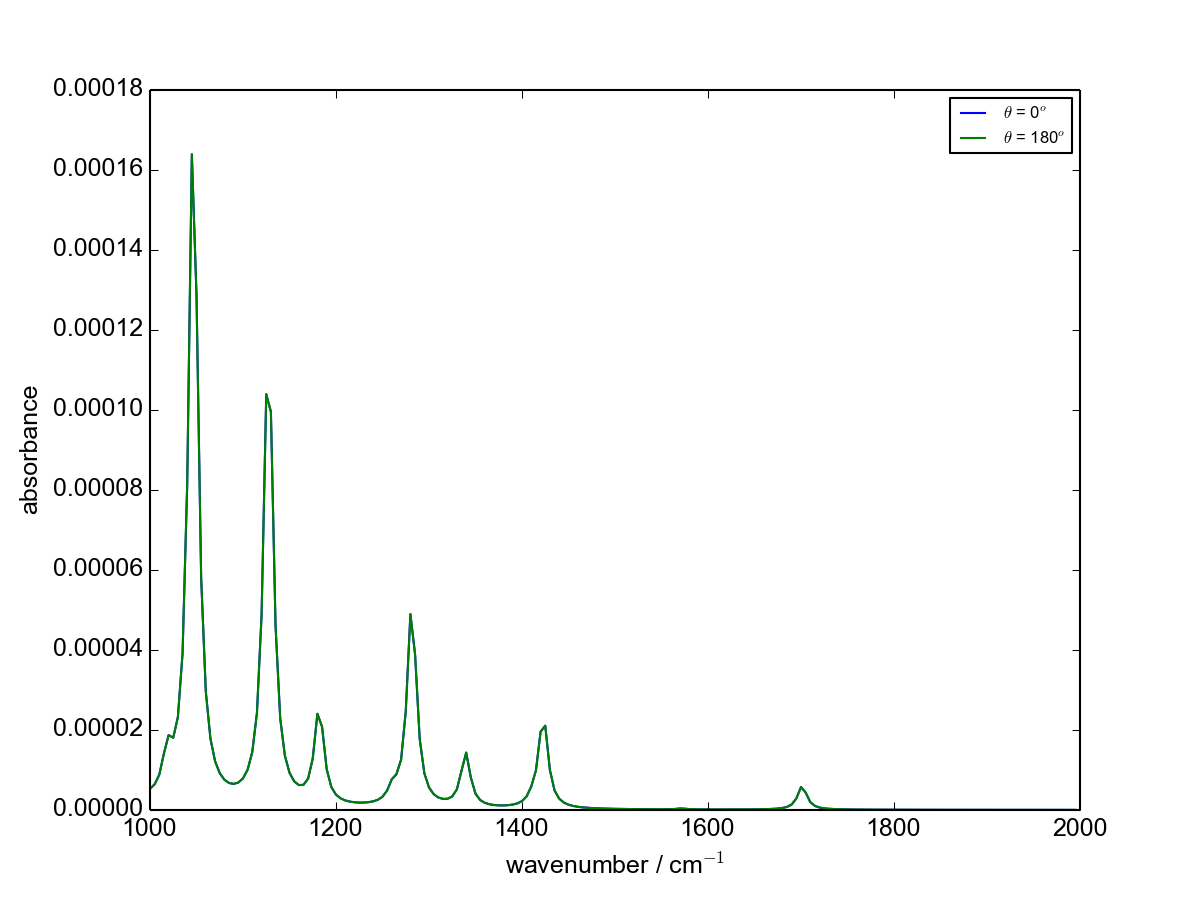
\includegraphics[scale=0.7]{Figures/Ala_candidates_plotting_ir_z_2.png}
\caption{IR $z$ projection spectrum for alanine candidate with $\theta$ of $0^{\circ}$ is identical to alanine candidate with $\theta$ of $180^{\circ}$.} \label{fig:A.1}
\end{figure}

\begin{figure}[!ht] 
\centering
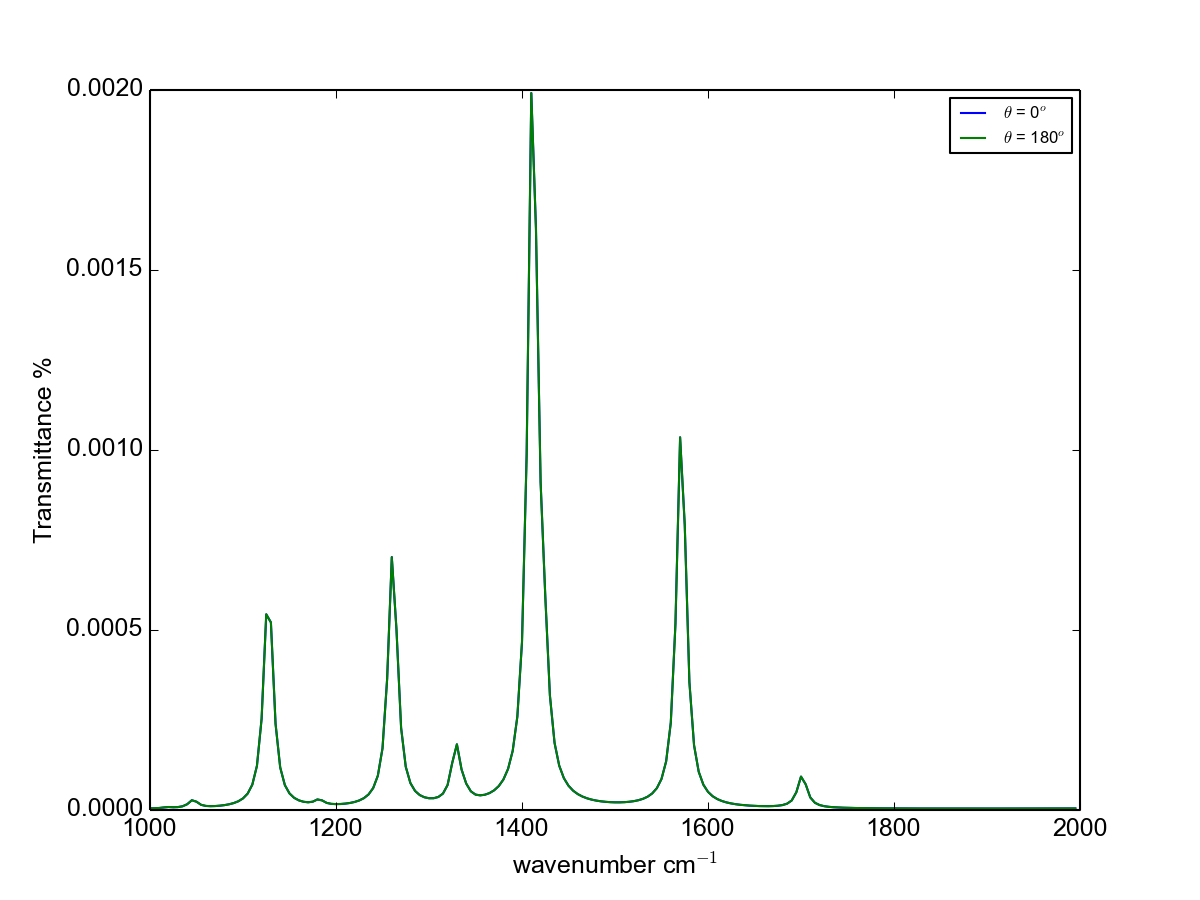
\includegraphics[scale=0.7]{Figures/Ala_candidates_plotting_raman_zz_2.png}
\caption{Raman $zz$ projection spectrum for alanine candidate with $\theta$ of $0^{\circ}$ is identical to alanine candidate with $\theta$ of $180^{\circ}$.} \label{fig:A.2}
\end{figure}

\begin{figure}[!ht] 
\centering
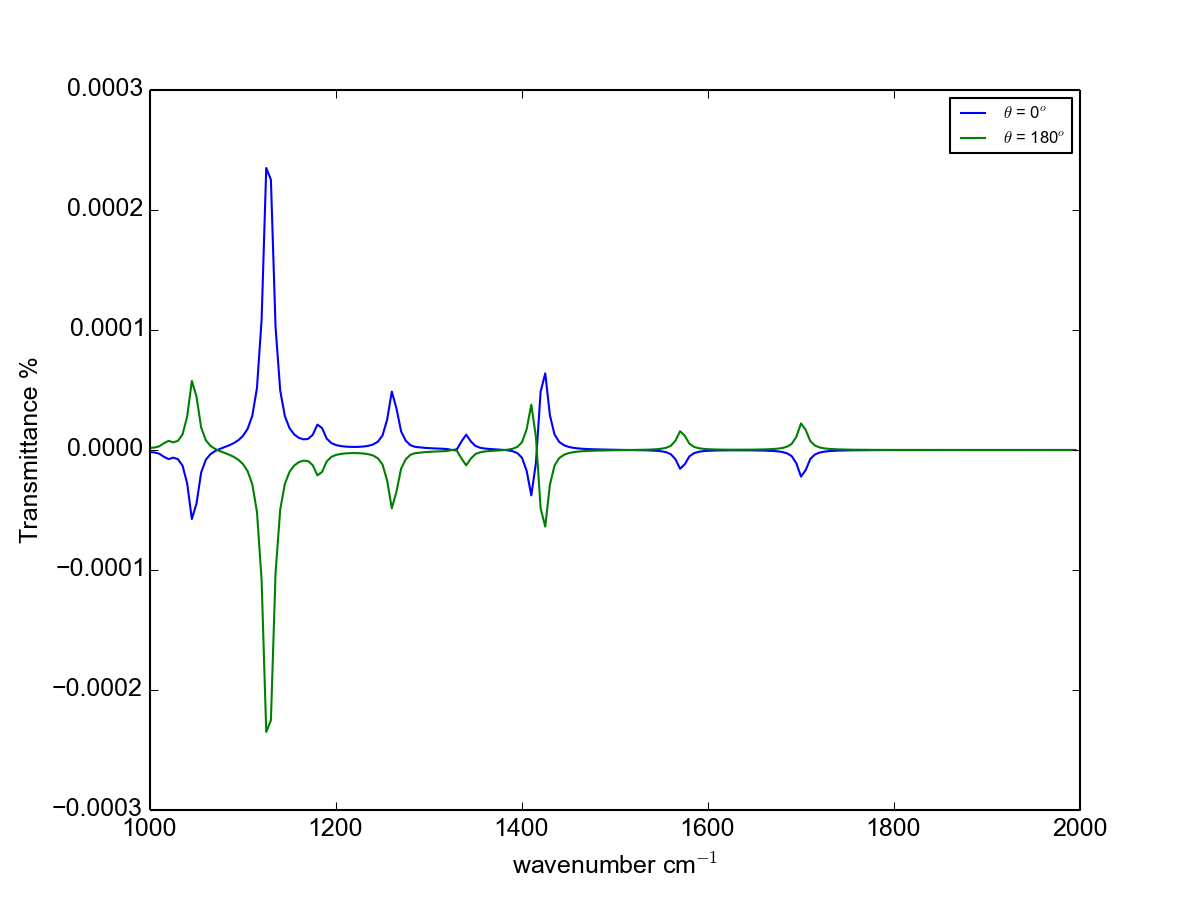
\includegraphics[scale=0.7]{Figures/Ala_candidates_plotting_sfg_zzz_2.png}
\caption{SFG $zzz$ projection spectrum for alanine candidate with $\theta$ of $0^{\circ}$ is not identical to alanine candidate with $\theta$ of $180^{\circ}$, but symmetric along wavelength.} 
\label{fig:A.3}
\end{figure}

\begin{table}[ht!] \tiny
\begin{center}
\resizebox{\textwidth}{!}{
\begin{tabular}{| l | p{3cm} | l | l |}
\hline
Number of Candidates & \multicolumn{2}{l|}{5} \\ \hline
Candidates & \multicolumn{2}{l|}{[0, 10, 20, 30, 40]} \\ \hline
Target Composition & \multicolumn{2}{l|}{[0.2, 0.2, 0.2, 0.2, 0.2]} \\ \hline
Test case index & Constraints & Result  \\ \hline
10 & 200, $x$ \newline 200, $z$& [0.607766, 0, 0, 0, 0.392234]  \\ \hline
11 & 200, $xx$ \newline 200, $xy$ \newline 200, $xz$ \newline 200, $zz$& [0.247792, 0, 0.502139, 0, 0.250069]  \\ \hline
12 & 200, $xxz$ \newline 200, $xzx$ \newline 200, $zzz$& [0.321014, 0, 0.31018, 0.163041, 0.205764]  \\ \hline
13 & 200, $x$ \newline 200, $z$ \newline 200, $xx$ \newline 200, $xy$ \newline 200, $xz$ \newline 200, $zz$& [0.247792, 0, 0.502139, 0, 0.250069]  \\ \hline
14 & 200, $xx$ \newline 200, $xy$ \newline 200, $xz$ \newline 200, $zz$ \newline 200, $xxz$ \newline 200, $xzx$ \newline 200, $zzz$& [0.321014, 0, 0.31018, 0.163041, 0.205764]  \\ \hline
15 & 200, $x$ \newline 200, $z$ \newline 200, $xxz$ \newline 200, $xzx$ \newline 200, $zzz$& [0.321014, 0, 0.31018, 0.163041, 0.205764]  \\ \hline
16 & 200, $x$ \newline 200, $z$ \newline 200, $xx$ \newline 200, $xy$ \newline 200, $xz$ \newline 200, $zz$ \newline 200, $xxz$ \newline 200, $xzx$ \newline 200, $zzz$& [0.321014, 0, 0.31018, 0.163041, 0.205764]  \\ \hline
\end{tabular} 
}
\end{center}
\caption{More detailed result data of Test Case 10 to 16 for methionine candidates.} \label{tab:7.1}
\end{table}

\begin{table}[ht!] 
\begin{center}
\resizebox{\textwidth}{!}{
\begin{tabular}{| l | p{3cm} | l | l }
\hline
\# Candidates & \multicolumn{2}{l|}{9} \\ \hline
Candidates & \multicolumn{2}{l|}{[0, 10, 20, 30, 40, 50, 60, 70, 80]} \\ \hline
Target Composition & \multicolumn{2}{l|}{[0.2201, 0.28905, 0.05201, 0.08251, 0.35633, 0, 0, 0, 0]} \\ \hline
Test Case \# & \# of Data Points & Result Composition \\ \hline
17 & each 5 wavenumber of IR, \newline Raman and SFG spectra & [0.158921, 0.388434, 0.0, 0.0985466, 0.354099, 0.0, 0.0, 0.0, 0.0] \\ \hline
18 & each 500 wavenumber of IR, \newline Raman and SFG spectra & [0.397991, 0.0, 0.203394, 0.0357663, 0.362848, 0.0, 0.0, 0.0, 0.0] \\ \hline
\end{tabular} 
}
\end{center}
\caption{More detailed result data of Test case 17 and 18 to explain the limitation of our LP model for methionine molecule.}
\label{tab:7.2}
\end{table}	

\begin{table}[ht!] \small
\begin{center}
{\def\arraystretch{1.5}
\begin{tabular}{| p{1cm} | p{3cm} | p{5cm} | l |} \hline
	Test Case \# & \# Data Points & Points Selection & Return Composition \\ \hline
	6 & 10 & [2800, 3300, 50], $z$ & [0, 0.796962, 0.103038, 0.1] \\ \hline
	7 & 20 & [2800, 3300, 25], $z$ & [0, 0.796962, 0.103038, 0.1] \\ \hline
	8 & 25 & [2800, 3300, 20], $z$ & [0, 0.796962, 0.103038, 0.1] \\ \hline
	9 & 32 & [2800, 3300, 15], $z$ & [0, 0.796962, 0.103038, 0.1] \\ \hline
	10 & 50 & [2800, 3300, 10], $z$ & [0, 0.796962, 0.103038, 0.1] \\ \hline
	11 & 100 & [2800, 3300, 5], $z$ & [0, 0.796962, 0.103038, 0.1] \\ \hline
	12 & $100 + 1$ & [2800, 3300, 5], $z$ \newline [2800, 3300, 500], $x$ & [0, 0.796962, 0.103038, 0.1] \\ \hline
	13 & $100 + 5$ & [2800, 3300, 20], $z$ \newline [2800, 3300, 100], $x$ & [0, 0.796962, 0.103038, 0.1] \\ \hline
	14 & $100 + 10$ & [2800, 3300, 20], $z$ \newline  [2800, 3300, 50], $x$ & [0, 0.796962, 0.103038, 0.1] \\ \hline
	15 & $100 + 50$ & [2800, 3300, 20], $z$ \newline  [2800, 3300, 10], $x$ & [0.1, 0.5, 0.4, 0] \\ \hline
	16 & $100 + 100$ & [2800, 3300, 20], $z$ \newline  [2800, 3300, 5], $x$ & [0.1, 0.5, 0.4, 0] \\ 
	\hline
\end{tabular} 
}
\end{center}
\caption{Constraint study based on Case 4 of simplified molecular model.} \label{tab:7.3}
\end{table}

\begin{table}[ht!] 
\begin{center} \tiny
{\def\arraystretch{1.5}
\begin{tabular}{| p{1cm} | p{2cm} | p{4cm}  | l |}
\hline
Test Case \# & \# of Data Points & Point Selection & Return Composition \\ \hline
17 & 10 & [2800, 3300, 50], $z$ & [0.156758, 0, 0, 0.825977, 0, 0, 0, 0, 0, 0.017265] \\ \hline
18 & 25 & [2800, 3300, 20], $z$ & [0, 0, 0.730541, 0, 0.212061, 0, 0, 0.0573978, 0, 0, 0] \\ \hline
19 & 50 & [2800, 3300, 10], $z$ & [0, 0, 0.730541, 0, 0.212061, 0, 0, 0.0573978, 0, 0, 0] \\ \hline
20 & 100 & [2800, 3300, 5], $z$ & [0, 0, 0.730541, 0, 0.212061, 0, 0, 0.0573978, 0, 0, 0] \\ \hline
21 & 500 & [2800, 3300, 1], $z$ & [0, 0, 0.730541, 0, 0.212061, 0, 0, 0.0573978, 0, 0, 0] \\ \hline	
22 & $100 + 1$ & [2800, 3300, 5], $z$ \newline [2800, 3300, 500], $x$  & [0, 0, 0.730541, 0, 0.212061, 0, 0, 0.0573978, 0, 0, 0] \\ \hline
23 & $100 + 10$ & [2800, 3300, 5], $z$ \newline [2800, 3300, 50], $x$  & [0.361587, 0, 0.312061, 0.326352, 0, 0, 0, 0, 0] \\ \hline
24 & $100 + 20$ & [2800, 3300, 5], $z$ \newline [2800, 3300, 25], $x$  & [0.174023, 0, 0, 0.791447, 0, 0, 0.0345301, 0, 0, 0] \\ \hline
25 & $100 + 25$ & [2800, 3300, 20], $z$ \newline [2800, 3300, 20], $x$  & [0.174023, 0, 0, 0.791447, 0, 0, 0.0345301, 0, 0, 0] \\ \hline
26 & $100 + 50$ & [2800, 3300, 5], $z$ \newline [2800, 3300, 10], $x$  & [0, 0, 0.753209, 0, 0.146791, 0, 0.1, 0, 0, 0] \\ \hline
27 & $100 + 84$ & [2800, 3300, 5], $z$ \newline [2800, 3300, 6], $x$  & [0.174023, 0, 0, 0.791447, 0, 0, 0.0345301, 0, 0, 0] \\ \hline
28 & $100 + 100$ & [2800, 3300, 5], $z$ \newline [2800, 3300, 5], $x$  & [0.1, 0, 0.5, 0, 0.4, 0, 0, 0, 0, 0] \\ 
\hline
\end{tabular} \\
}
\caption{Constraint study based on Case 5 of simplified molecular model.}\label{tab:7.4}
\end{center}
\end{table}